\section{Appendix}

\begin{figure*}
    \centering
%    \begin{subfigure}{0.3\linewidth}
%        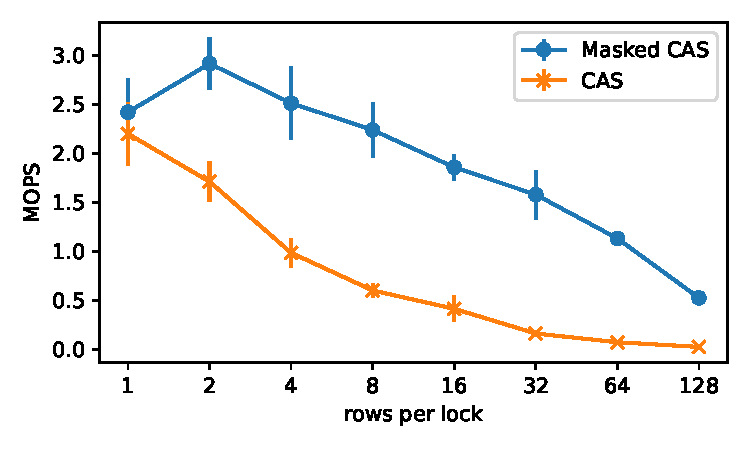
\includegraphics[width=0.99\linewidth]{fig/masked_cas_lock_size.pdf}
%    \end{subfigure}
    \begin{subfigure}{0.45\linewidth}
        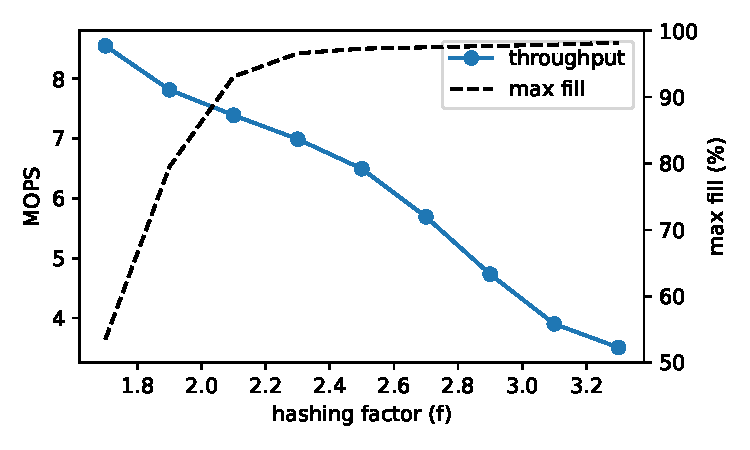
\includegraphics[width=0.99\linewidth]{fig/factor.pdf}
        % \label{fig:hash_fill}
        % \caption{}
    \end{subfigure}
    \begin{subfigure}{0.45\linewidth}
        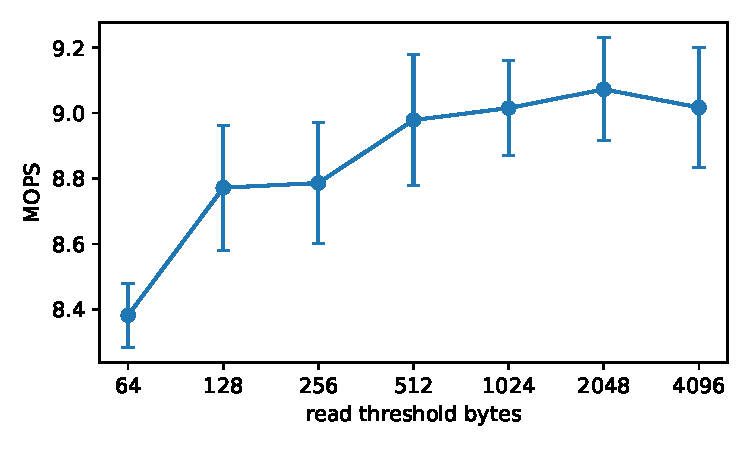
\includegraphics[width=0.99\linewidth]{fig/read_size.pdf}
        % \label{fig:hash_factor}
        % \caption{}
    \end{subfigure}
    %\begin{figure}[ht]
    % \begin{subfigure}{0.3\linewidth}
    %   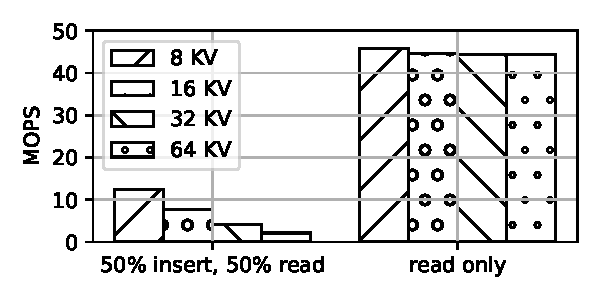
\includegraphics[width=0.99\linewidth]{fig/entry_size.pdf}
    %       \end{subfigure}
%    \caption{Throughput vs KV entry size}

%\end{figure}
    \vspace{-1em}
    \caption{RCuckoo parameter sweeps:
      \textbf{(a)} Throughput and max fill vs locality factor,
          \textbf{(b)} throughput vs read threshold, and 
    \textbf{(c)} throughput vs key/value entry size.
    }
    \label{fig:performance_breakdown}
             \label{fig:entry_size}
\end{figure*}


\textbf{Locality factor.}  The left-most graph shows that lower hash
factors $f$ deliver higher performance (plotted against the left axis)
due to better locality at the cost of lower expected maximum fill
factors (right axis).
%the tradeoff of their maximum fill factor. The
%relationship between $f$ and performance is nearly linear, while the
%relationship between $f$ and fill factor is
%exponential. Figure~\ref{fig:performance_breakdown}(c) shows the
%relationship between $f$, the max fill rate, and insert
%performance. These numbers were collected on an
This experiment consists of an insert-only workload (YCSB-W)
on a 100-M entry table. We choose an $f$ of 2.3 in practice as
it has the highest product of fill factor and throughput.
\todo{Section 4 says we use an f of 2.1?}

\textbf{Read threshold.}
\label{sec:read_threshold}
%As described in Section~\ref{sec:reading}
RCuckoo issues a covering
read if both key locations are within a defined threshold (128 bytes
in our experiments) of each other.
Figure~\ref{fig:performance_breakdown}(b) shows that performance
increases with larger thresholds, but at the cost of additional
bandwidth consumption.  In this experiment, only 40 clients
access a table with 64-byte rows, so they do not exhaust link bandwidth even with a 4-KB covering read, but performance levels off after 2 KB.
%% performance gains from increasing the read threshold. Here
%% each row is 64 bytes so our minimum threshold of 64 ensures
%% two packets are issued for each read request. We limit the
%% number of clients to 40 so that their is plenty of bandwidth
%% to support the inflated reads. Higher read thresholds trade
%% off network bandwidth for operation latency. 
Under these conditions, if bandwidth is plentiful larger (i.e., 2-KB
vs 128-B) covering reads can improve throughput, but only modestly.
%8\%.

% \begin{figure}[ht]
%     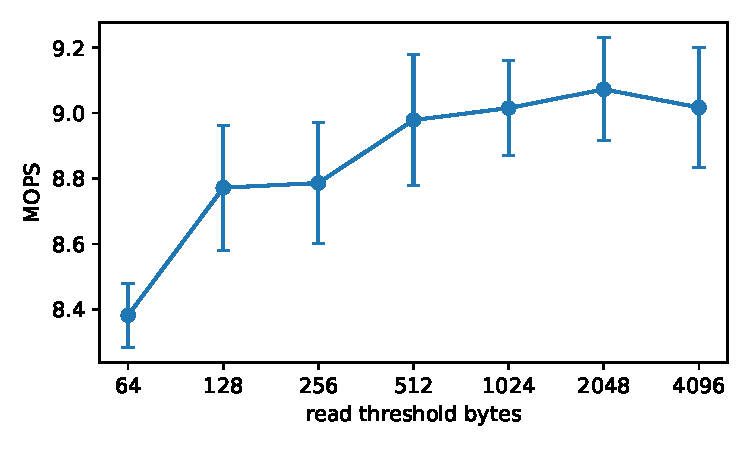
\includegraphics[width=0.99\linewidth]{fig/read_size.pdf}
%     \caption{Read Threshold vs Throughput}
%     \label{fig:read_threshold}
% \end{figure}